\section{Background}
\subsection{Background of distributed query execution}
The architecture and terms are instroduced in this section to serve the as basis for the further discussions. 
The figure~\ref{fig:architecture} demonstrates how a query is processed by a distributed query system. In this case, we use the Hadoop2.0(HIive+Tez architecture) as an example.

\begin{figure}[t]
	\centering
	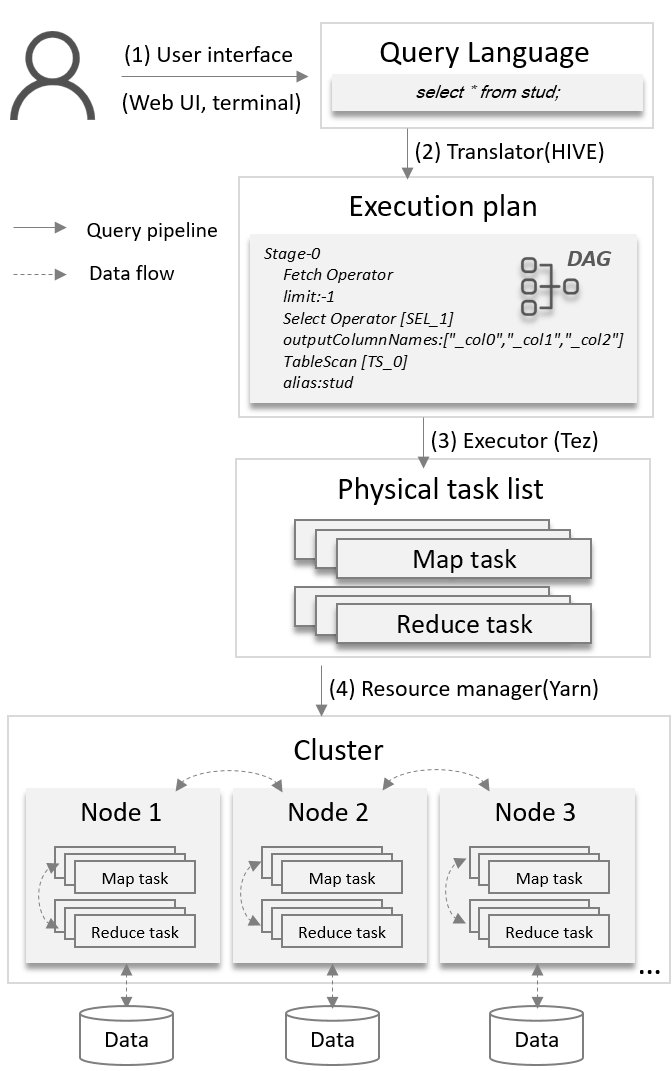
\includegraphics[width=0.40\textwidth]{figures/background/arc.png}
	\vspace{-3mm}
	\caption{Overview of Hive2.0 distributed query architecture.}
	\label{fig:architecture}
	\vspace{-3mm}
\end{figure}


\begin{figure}[t]
	\centering
	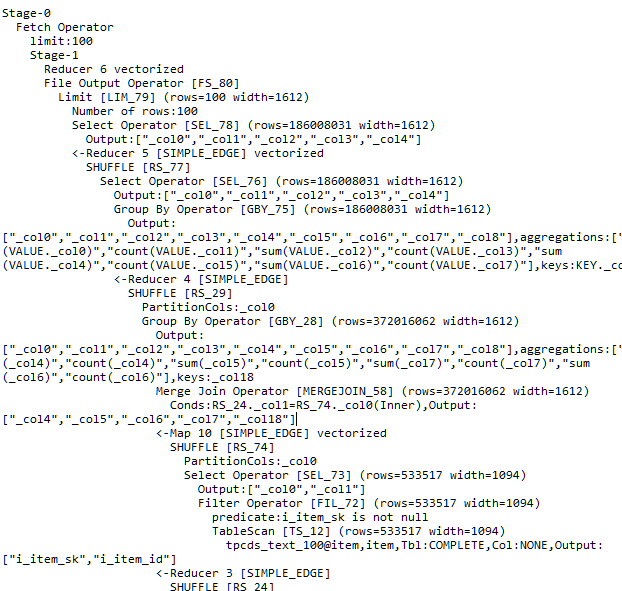
\includegraphics[width=0.45\textwidth]{figures/background/execution_plan.png}
	\vspace{-3mm}
	\caption{The hive execution plan.}
	\label{fig:exec_plan}
	\vspace{-3mm}
\end{figure}

When user issues a query (shown as Figure~\ref{fig:architecture}(1)) through the interface such as a web UI or SQL terminal, Hive optimizes it and translate it as the detail logic execution plan shown as Figure~\ref{fig:architecture}. The logic exaction plan may contains hundreds of lines of description, which usually describe the execution process as a Directed Acyclic Graph(DAG). The DAG includes two types of vertex: map vertex and reduce vertex. Each vertex contains a sequence of logic operators such as filter, aggregate, merge, etc. Moreover, there are edges connecting the verteices. The edges define the data movement between vertecies, the source vertices are the producers and the destinat vertices are the consumers.
Tez further generates the physical tasks according to the work flow of vertices and YARN dispatches these tasks on the Hadoop worker machines.  The task is the atomic process of the query. All tasks of the a specific vertex are dispatched to multiple machines and processed according to operators of the vertex.  

\subsection{Requirement analysis}
During the one year of collaboration, we have closely collaborated with three experts in distributed database, who are also the co-authors of this paper.

In the first month of the collaboration, we have held brainstorming to collect the most frequent raised questions when analyzing the distributed query system performance. Based the discussions with domain experts and review of existing literature, we have formulated the following design requirements.

\textbf{R1.Understand the general query execution trace and query plan structure.} Before our collaboration, the domain experts have used profiling software (TezVIS, etc) or visualization tools(Tableau, etc) to show the query progress as Ganntt chart and query plan structure as directed graph. However, these two visualizations are always displayed in separated views which require users to switch their focus and break the continuity of exploration. Is it possible to  integrate these two visualization forms into one view thus to keep the continuity of exploration?

\textbf{R2.Understand the query process at the task level.}
Understand the execution of single task can be helpful to identify the bottleneck of the whole query process.
However, visualize the tasks is challenge. First, to visualize the tasks in traditional way(Gantt diagram) need a large canvas. The multiple features such as the size of data and the operators should be visualized for understanding the task. Moreover, the many to many relationship among the tasks also makes it difficult to design clear and \textbf{scaleble} visualization.

\textbf{R3.Provide the visual insight to reason the behaviour and pattern of a specific task.}
To solely visualize the tasks themselves are not enough to explain the specific pattern of tasks. Many reason about the hardware resource such as the network status, hard disk waiting list is also related to the patterns. Such kinds of information should be vitalized effectively to assist the exploration of query executions. 

\textbf{R4.Provide the flexible interactions allowing users to switch the focus among different point of interest, enable users to facilitate the multi-level of explorations.}
Other than the visualization designs, a flexible interaction should be implemented for users to navigate to any point of interest. The linkage among the correlated visual elements are also should be designed to coordinate the information.